\label{Chapter_3}
\section{Methodology for Review of Literature}
\label{sec:review-method}
A defensible account of where existing security architectures fall short of the requirements set out in Section~\ref{sec:case} cannot rest on a selective reading of convenient sources. It requires a search that is reproducible, criteria that are stated in advance, and a corpus assembled without the bias that undermines a narrative survey. The review reported in this chapter therefore adopts the Preferred Reporting Items for Systematic Reviews and Meta-Analyses (PRISMA) framework~\cite{prisma}, which prescribes a transparent, stage-by-stage procedure for identifying, screening, and selecting studies and for reporting the exclusions made at each stage. The phenomenon of interest is the intersection at which the thesis is positioned: learning-driven detection, blockchain-anchored provenance, and post-quantum protection, examined under the resource constraints of industrial deployment rather than in the abstract.

The search was conducted across five databases, namely IEEE Xplore, Scopus, Web of Science, the ACM Digital Library, and SpringerLink, between 1 March and 5 April 2025, targeting publications from 2020 to 2025. Restricting the corpus to this window is deliberate rather than incidental: the convergence of hybrid ledgers, learning-based security, and post-quantum standardisation that the thesis addresses emerged substantially within this period, so an earlier window would dilute relevance rather than improve coverage. Six core terms structured the query, namely ``hybrid blockchain'', ``digital twin'', ``data-sharing security'', ``cross-chain'', ``privacy-preserving blockchain'', and ``energy-efficient consensus'', each adapted to the query syntax of the individual databases. Table~\ref{tab:search-strings} records the exact string issued to each database, so that the search can be reproduced rather than merely described.

\subsection{Inclusion and Exclusion Criteria}
\label{subsec:review-criteria}

Eligibility was decided against criteria fixed before screening began, so that inclusion reflected the protocol rather than the reviewer's expectation. A study was included if it satisfied all of the following:
\begin{itemize}
  \item published in a peer-reviewed journal or conference proceedings;
  \item published within the 2020 to 2025 window;
  \item directly concerned with hybrid blockchain technology in the context of secure, resource-aware data sharing;
  \item written in English.
\end{itemize}
A study was excluded if it lacked conceptual depth, reported neither empirical nor analytical validation, or addressed blockchain applications outside the defined scope. Non-original items such as editorials and letters were removed without further assessment.

\subsection{Article Selection Results}
\label{subsec:review-results}

The search returned 512 records. Automated and manual deduplication reduced these to 412 unique records. Screening of titles and abstracts removed 162 irrelevant publications, leaving 250 for full-text assessment, of which 134 were excluded for insufficient conceptual depth, absence of validation, or scope mismatch. The final corpus comprised 116 studies, 99 of them quantitative and 17 qualitative. Figure~\ref{fig:prisma-flow} presents the complete PRISMA selection flow, with the count retained and the reasons for exclusion recorded at each stage.

The composition of the retained corpus locates the field in time and domain. Studies published in 2023 and 2024 account for 62 of the 116 works, a little over half, which confirms the rapid growth of the area; 2021 and 2022 contribute 29 works, and 2020 together with 2025 the remaining 25. Peer-reviewed journal articles dominate the corpus, with conference proceedings and book chapters forming a smaller share, indicating a research area maturing toward archival publication. By application domain, healthcare and the Internet of Medical Things, industrial and cyber-physical systems, transport and the Internet of Vehicles, and energy systems are the most frequently addressed, with construction, supply chain, and civic systems adding further diversity and the remainder spanning multi-domain or general settings. Figure~\ref{fig:review-stats} summarises this distribution.

\subsection{Quality Assessment and Bias Evaluation}
\label{subsec:review-quality}

Each retained study was assessed against five quality criteria: clarity of research objectives; reproducibility of the proposed method or system design; traceability of results, meaning whether performance claims such as throughput, latency, or energy efficiency were supported by experimental data or formal analysis; relevance to hybrid blockchain and resource-aware data sharing; and acknowledgement of study-level limitations. Failure on objectives, reproducibility, or relevance was grounds for exclusion at full-text review.

Five sources of bias were addressed directly rather than left implicit. Publication bias was mitigated by spanning five databases across multiple publishers and venues. Language bias is acknowledged, since the English-only restriction may omit relevant non-English work, although English dominates peer-reviewed research in this area over the target period. Selection bias was controlled by applying the inclusion and exclusion criteria consistently across both screening phases, with ambiguous cases resolved by re-evaluation. Recency bias is inherent to the 2020 to 2025 scope but deliberate, given that the field emerged largely within it. Aggregation bias, arising from heterogeneous performance metrics across studies, is acknowledged as a residual limitation: every quantitative figure carried into this review is attributed to its primary source and is not treated as a cross-study validated or normalised estimate.

% ---------------------------------------------------------------------
% TABLE 3.x — search strings per database (reproduce from the DT paper's Table 3)
% ---------------------------------------------------------------------
\begin{table}[t]
  \centering
  \footnotesize
  \setlength{\tabcolsep}{4pt}
  \renewcommand{\arraystretch}{1.3}
  \caption{Search string issued to each database, adapted to the query syntax of the source.}
  \label{tab:search-strings}
  \begin{tabularx}{\columnwidth}{@{}
      >{\raggedright\arraybackslash}p{2.4cm}
      >{\raggedright\arraybackslash}X@{}}
    \toprule
    \textbf{Database} & \textbf{Search string} \\
    \midrule
    IEEE Xplore   & (``digital twin'' OR ``DT'') AND (``hybrid blockchain'' OR ``public private blockchain'') AND (security OR privacy OR interoperability) \\
    \addlinespace
    Scopus        & TITLE-ABS-KEY(``digital twin'' AND ``hybrid blockchain'') AND (privacy OR security OR consensus) \\
    \addlinespace
    Web of Science & TS=(``digital twin'' AND ``hybrid blockchain'') AND TS=(security OR privacy) \\
    \addlinespace
    ACM DL        & [[Abstract: ``digital twin''] AND [``hybrid blockchain'']] AND [keywords: security OR consensus] \\
    \addlinespace
    SpringerLink  & (``digital twin'' + ``hybrid blockchain'' + security OR privacy) in Title or Abstract \\
    \bottomrule
  \end{tabularx}
\end{table}

\begin{figure}[t]
  \centering
  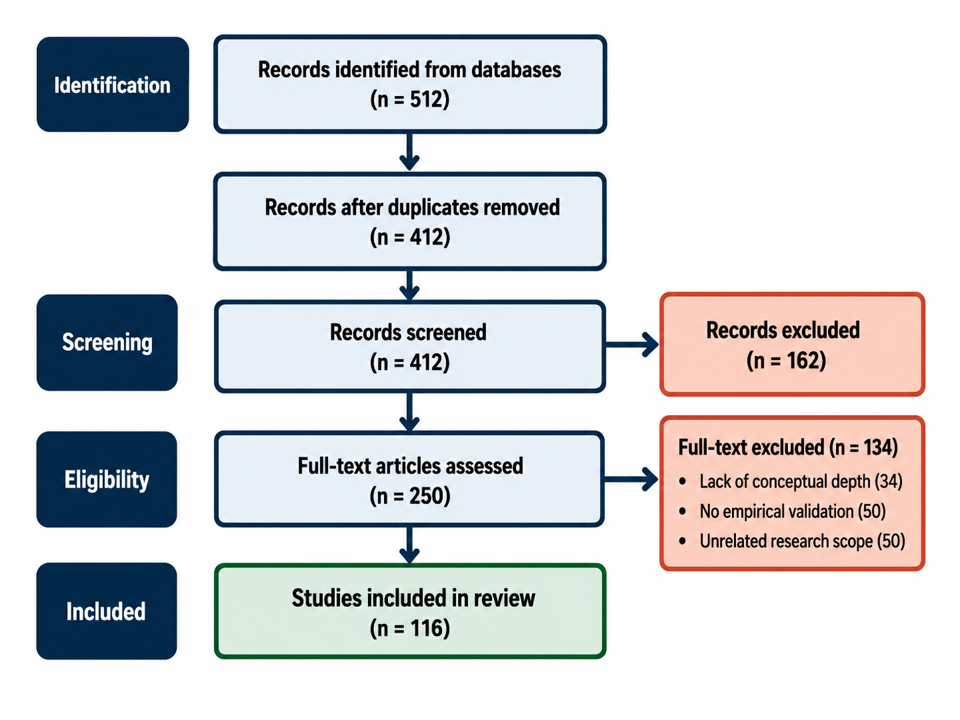
\includegraphics[width=0.9\columnwidth]{figures/Picture11.png}
  \caption{PRISMA 2020 flow diagram showing record identification, screening, eligibility assessment, and inclusion, with the count retained and the reason for exclusion recorded at each stage: 512 records identified, 412 after deduplication, 250 after title and abstract screening, and 116 retained after full-text assessment.}
  \label{fig:prisma-flow}
\end{figure}


\begin{figure}[t]
  \centering
  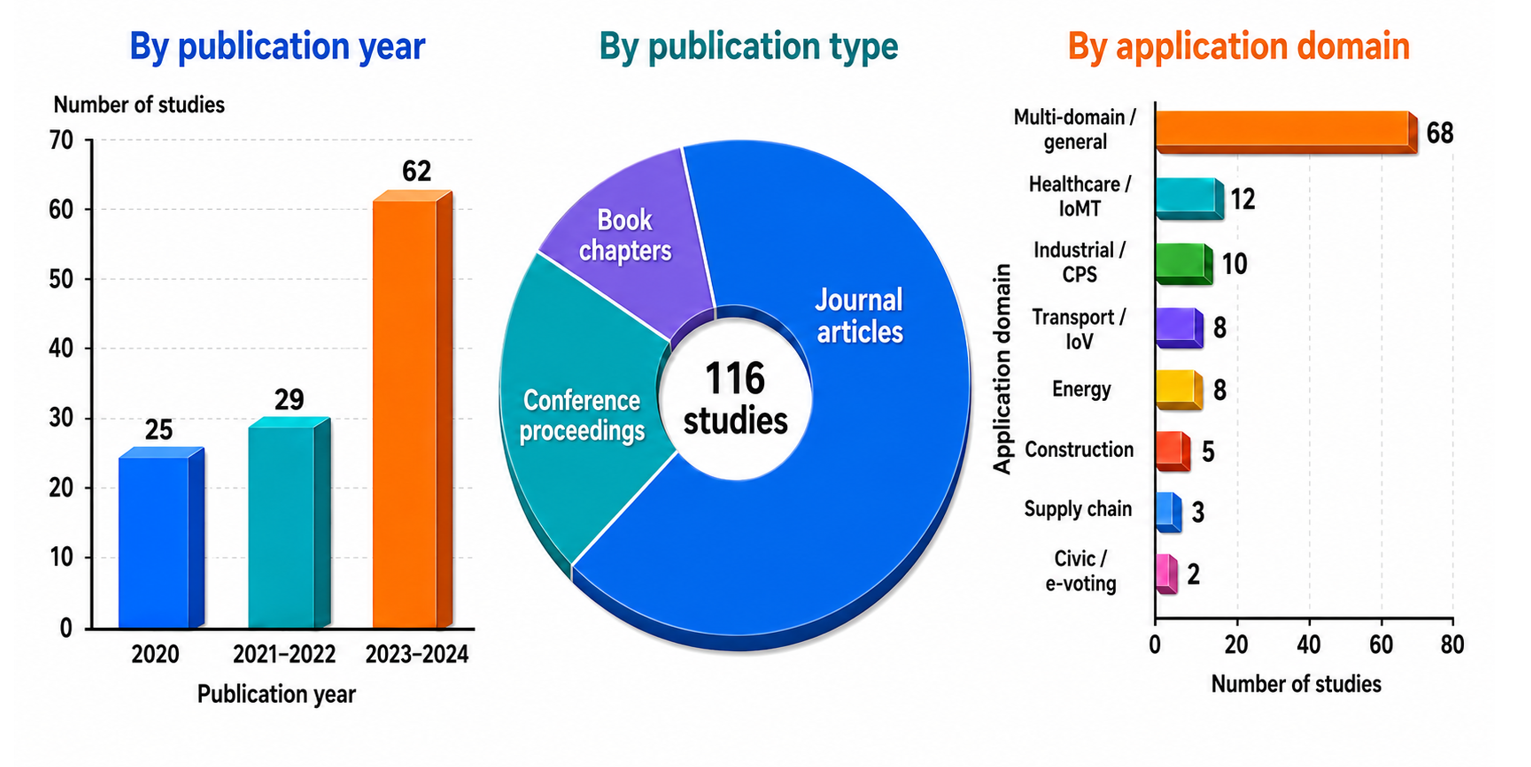
\includegraphics[width=0.97\columnwidth]{figures/Picture122.png}
   \caption{Distribution of the 116 retained studies. Left: by publication year, with more than half of the corpus published in 2023 and 2024. Right: by application domain, with the seven most frequently addressed specific domains shown and the remaining studies grouped as multi-domain or general contexts. By publication type, peer-reviewed journal articles dominate the corpus, with conference proceedings and book chapters forming a smaller share.}
    \label{fig:review-stats}
\end{figure}


 
\section{Review of Recent Works}
\label{sec:recent-works}
 
Substantial effort has been directed at securing blockchain-enabled and digital-twin systems, and a first orientation is best obtained not from individual proposals but from the reviews that have already synthesised them. Table~\ref{tab:review-comparison} compares the most relevant prior review and survey works along the dimensions that decide whether a review speaks to the problem addressed here: whether it treats the digital-twin ecosystem (DTE) as its object, whether it engages conventional blockchain technology (CBT) or the hybrid model (HBT), whether it organises its findings through a three-dimensional lifecycle-layer-security taxonomy, whether it performs a comparative defence-gap analysis, and whether it traces each open issue to a research direction. The final three columns tell the decisive story at a glance: across every prior review, the taxonomy, defence-gap, and issue-to-direction columns are uniformly absent, and only the present review supplies all three.
 
The prior reviews fall into three groups, each capable within its remit and each limited in the same structural way. The first group treats blockchain as a broad enabler of digital twins without isolating the hybrid model as a necessary architectural response. Surveys of blockchain for digital twins~\cite{yaqoob}, of blockchain-based digital-twin trends~\cite{sabah}, of digital-twin and blockchain integration~\cite{hemdan}, and the more recent multi-domain accounts~\cite{dwivedi,Nexus} cover the pairing of the two technologies capably, but treat the choice between public, private, and hybrid ledgers as a design detail rather than as the structural pivot on which digital-twin security turns. The second group narrows to the hybrid model but not to the digital-twin setting: the one prior systematic review of hybrid blockchain platforms~\cite{alkhateeb} addresses general Internet-of-Things systems and does not engage the lifecycle-specific trade-offs that arise under real-time, high-frequency workloads. The third group reviews digital-twin architecture and enabling technologies thoroughly, in accounts of digital-twin technology and networking~\cite{maggie}, of enabling technologies and prospects~\cite{Mihai}, and of Internet-of-Digital-Twins architecture~\cite{wangbest}, but offers no security-focused synthesis, no defence-gap analysis, and no structured mapping from open issue to future direction.
 
A closer reading within these groups reinforces the point. The domain-specific reviews demonstrate real depth in their settings, of digital twins in remanufacturing supply chains~\cite{chen}, of blockchain for secure health data sharing~\cite{peng,upadrista}, of building-lifecycle management~\cite{adu}, of security in Industry~4.0 digital twins~\cite{elhajj}, and of data fusion in the energy sector~\cite{jiang}, yet their security treatment stays bound to the application rather than abstracted into a reusable architectural principle. The recent multi-domain reviews extend coverage and currency, and one adds case-study evidence alongside its systematic method~\cite{christos,Nexus}, but none introduces the three analytical dimensions on which a trust-partitioned architecture must be assessed. Several of these works are systematic in method~\cite{chen,alkhateeb,upadrista,adu,christos,Nexus,elhajj,jiang}, which confirms that methodological rigour is not what the field lacks; what it lacks is a security-focused synthesis organised around the hybrid, trust-partitioned model.
 
Read together, these reviews establish that the field has matured and that the pairing of blockchain with digital-twin and industrial systems is now well surveyed. What none provides, as the three rightmost columns of Table~\ref{tableX} make explicit, is a security-focused synthesis that isolates the hybrid, trust-partitioned model as a structural response, measures the defence coverage it achieves, and traces the residual gaps to the directions that would close them. That absence defines the contribution of the review reported here. The substantive state of the art on which it draws is examined next in Section~\ref{sec:soa}, before the resulting gaps are consolidated in Section~\ref{sec:review-gap}.

\begin{table*}[!htbp]
\centering
\setlength{\arrayrulewidth}{0.8mm}
\caption{Comparison of Selected Related Works}
\resizebox{\textwidth}{!}{%
\begin{tabular}{llllccccccccc}
\hline
\textbf{Ref} & \textbf{Year} & \textbf{Review Target Area} & \textbf{Review Remarks} & \textbf{Systematic Review} & \textbf{Case Studies} & \textbf{DTE} & \textbf{CBT} & \textbf{HBT} & \textcolor{black}{\textbf{3D Tax.}} & \textcolor{black}{\textbf{Defense Gap}} & \textcolor{black}{\textbf{Issue--Dir. Trace.}} \\
\hline
\cite{yaqoob} & 2020 & Non-specific & Secure manufacturing & \ding{55} & \checkmark & \checkmark & \checkmark & \ding{55} & \ding{55} & \ding{55} & \ding{55} \\
\midrule
\cite{maggie} & 2021 & Non-specific & Technology of DT & \ding{55} & \ding{55} & \checkmark & \ding{55} & \ding{55} & \ding{55} & \ding{55} & \ding{55} \\
\midrule
\cite{chen} & 2021 & Supply chains & DT in remanufacturing & \checkmark & \ding{55} & \checkmark & \ding{55} & \ding{55} & \ding{55} & \ding{55} & \ding{55} \\
\midrule
\cite{peng} & 2022 & Health & BT secure data sharing & \ding{55} & \ding{55} & \ding{55} & \checkmark & \ding{55} & \ding{55} & \ding{55} & \ding{55} \\
\midrule
\cite{alkhateeb} & 2022 & IoT & Adoption of HBT & \checkmark & \ding{55} & \ding{55} & \ding{55} & \checkmark & \ding{55} & \ding{55} & \ding{55} \\
\midrule
\cite{Mihai} & 2022 & Non-specific & Realization of DT & \ding{55} & \checkmark & \checkmark & \ding{55} & \ding{55} & \ding{55} & \ding{55} & \ding{55} \\
\midrule
\cite{sabah} & 2022 & Non-specific & Blockchain-based DT & \ding{55} & \ding{55} & \checkmark & \checkmark & \ding{55} & \ding{55} & \ding{55} & \ding{55} \\
\midrule
\cite{RUI} & 2023 & Non-specific & BT-based data sharing & \ding{55} & \ding{55} & \ding{55} & \checkmark & \ding{55} & \ding{55} & \ding{55} & \ding{55} \\
\midrule
\cite{hemdan} & 2023 & IoT Systems & DT and BT integration & \ding{55} & \ding{55} & \checkmark & \checkmark & \ding{55} & \ding{55} & \ding{55} & \ding{55} \\
\midrule
\cite{upadrista} & 2023 & Health & BT for data sharing & \checkmark & \ding{55} & \ding{55} & \checkmark & \ding{55} & \ding{55} & \ding{55} & \ding{55} \\
\midrule
\cite{wangbest} & 2023 & Non-specific & IoDT architecture & \ding{55} & \ding{55} & \checkmark & \ding{55} & \ding{55} & \ding{55} & \ding{55} & \ding{55} \\
\midrule
\cite{adu} & 2023 & Post-construction & Building management & \checkmark & \ding{55} & \checkmark & \checkmark & \ding{55} & \ding{55} & \ding{55} & \ding{55} \\
\midrule
\cite{dwivedi} & 2024 & Multi-domain & BT enabled DT & \ding{55} & \ding{55} & \checkmark & \checkmark & \ding{55} & \ding{55} & \ding{55} & \ding{55} \\
\midrule
\cite{christos} & 2024 & Smart Industry & BT and DT integration & \checkmark & \checkmark & \checkmark & \checkmark & \ding{55} & \ding{55} & \ding{55} & \ding{55} \\
\midrule
\cite{Nexus} & 2024 & Multi-domain & Effects of BT on DT & \checkmark & \ding{55} & \checkmark & \checkmark & \ding{55} & \ding{55} & \ding{55} & \ding{55} \\
\midrule
\cite{elhajj} & 2024 & Industry 4.0 & Security in DT & \checkmark & \ding{55} & \checkmark & \ding{55} & \ding{55} & \ding{55} & \ding{55} & \ding{55} \\
\midrule
\cite{jiang} & 2024 & Energy sector & Data fusion with DT & \checkmark & \ding{55} & \checkmark & \ding{55} & \ding{55} & \ding{55} & \ding{55} & \ding{55} \\
\midrule
\textbf{Ours} & \textbf{2026} & \textbf{Multi-domain} & \textbf{HBT secure data sharing} & \checkmark & \checkmark & \checkmark & \checkmark & \checkmark & \checkmark & \checkmark & \checkmark \\
\hline
\end{tabular}}
\label{tableX}
\scriptsize
\checkmark~Considered; $\times$~Not considered; \textcolor{black}{DTE: Digital Twin Ecosystem; CBT: Conventional Blockchain Technology; BT: Blockchain Technology; HBT: Hybrid Blockchain Technology.} \textcolor{black}{3D Tax.: Three-dimensional lifecycle-layer-security taxonomy; Defense Gap: Comparative defense coverage and residual gap analysis; Issue--Dir.~Trace.: Explicit open-issue to future research direction traceability.}
\end{table*}



\begin{sidewaystable}
\centering
\caption{Comparison of selected prior review works.}
\label{tab:review-comparison}
\renewcommand{\arraystretch}{1.25}
\setlength{\tabcolsep}{6pt}
\begin{tabular}{@{}l l l l cccccccc@{}}
\toprule
\textbf{Ref} & \textbf{Year} & \textbf{Target Area} & \textbf{Review Remarks}
 & \rotatebox{90}{\textbf{Systematic review}}
 & \rotatebox{90}{\textbf{Case study}}
 & \rotatebox{90}{\textbf{DTE}}
 & \rotatebox{90}{\textbf{CBT}}
 & \rotatebox{90}{\textbf{HBT}}
 & \rotatebox{90}{\textbf{3D Tax.}}
 & \rotatebox{90}{\textbf{Defence gap}}
 & \rotatebox{90}{\textbf{Issue--Dir.}} \\
\midrule
\cite{yaqoob}    & 2020 & Non-specific      & Secure manufacturing   & \ding{55} & \checkmark & \checkmark & \checkmark & \ding{55} & \ding{55} & \ding{55} & \ding{55} \\
\cite{maggie}    & 2021 & Non-specific      & Technology of DT       & \ding{55} & \ding{55} & \checkmark & \ding{55} & \ding{55} & \ding{55} & \ding{55} & \ding{55} \\
\cite{chen}      & 2021 & Supply chains     & DT in remanufacturing  & \checkmark & \ding{55} & \checkmark & \ding{55} & \ding{55} & \ding{55} & \ding{55} & \ding{55} \\
\cite{peng}      & 2022 & Health            & BT secure data sharing & \ding{55} & \ding{55} & \ding{55} & \checkmark & \ding{55} & \ding{55} & \ding{55} & \ding{55} \\
\cite{alkhateeb} & 2022 & IoT               & Adoption of HBT        & \checkmark & \ding{55} & \ding{55} & \ding{55} & \checkmark & \ding{55} & \ding{55} & \ding{55} \\
\cite{Mihai}     & 2022 & Non-specific      & Realization of DT      & \ding{55} & \checkmark & \checkmark & \ding{55} & \ding{55} & \ding{55} & \ding{55} & \ding{55} \\
\cite{sabah}     & 2022 & Non-specific      & Blockchain-based DT    & \ding{55} & \ding{55} & \checkmark & \checkmark & \ding{55} & \ding{55} & \ding{55} & \ding{55} \\
\cite{RUI}       & 2023 & Non-specific      & BT-based data sharing  & \ding{55} & \ding{55} & \ding{55} & \checkmark & \ding{55} & \ding{55} & \ding{55} & \ding{55} \\
\cite{hemdan}    & 2023 & IoT Systems       & DT and BT integration  & \ding{55} & \ding{55} & \checkmark & \checkmark & \ding{55} & \ding{55} & \ding{55} & \ding{55} \\
\cite{upadrista} & 2023 & Health            & BT for data sharing    & \checkmark & \ding{55} & \ding{55} & \checkmark & \ding{55} & \ding{55} & \ding{55} & \ding{55} \\
\cite{wangbest}  & 2023 & Non-specific      & IoDT architecture      & \ding{55} & \ding{55} & \checkmark & \ding{55} & \ding{55} & \ding{55} & \ding{55} & \ding{55} \\
\cite{adu}       & 2023 & Post-construction & Building management     & \checkmark & \ding{55} & \checkmark & \checkmark & \ding{55} & \ding{55} & \ding{55} & \ding{55} \\
\cite{dwivedi}   & 2024 & Multi-domain      & BT enabled DT          & \ding{55} & \ding{55} & \checkmark & \checkmark & \ding{55} & \ding{55} & \ding{55} & \ding{55} \\
\cite{christos}  & 2024 & Smart Industry    & BT and DT integration  & \checkmark & \checkmark & \checkmark & \checkmark & \ding{55} & \ding{55} & \ding{55} & \ding{55} \\
\cite{Nexus}     & 2024 & Multi-domain      & Effects of BT on DT    & \checkmark & \ding{55} & \checkmark & \checkmark & \ding{55} & \ding{55} & \ding{55} & \ding{55} \\
\cite{elhajj}    & 2024 & Industry 4.0      & Security in DT         & \checkmark & \ding{55} & \checkmark & \ding{55} & \ding{55} & \ding{55} & \ding{55} & \ding{55} \\
\cite{jiang}     & 2024 & Energy sector     & Data fusion with DT    & \checkmark & \ding{55} & \checkmark & \ding{55} & \ding{55} & \ding{55} & \ding{55} & \ding{55} \\
\midrule
\textbf{This review} & \textbf{2026} & \textbf{Multi-domain} & \textbf{Trust-partitioned security} & \checkmark & \checkmark & \checkmark & \checkmark & \checkmark & \checkmark & \checkmark & \checkmark \\
\bottomrule
\end{tabular}

\vspace{4pt}
{\footnotesize \checkmark~considered; $\times$~not considered.
DTE: digital-twin ecosystem; CBT: conventional blockchain technology; BT: blockchain technology; HBT: hybrid blockchain technology; 3D Tax.: three-dimensional lifecycle-layer-security taxonomy; Defence gap: comparative defence coverage and residual-gap analysis; Issue--Dir.: open-issue to future-direction traceability.}
\end{sidewaystable}



\section{State-of-the-Art Approaches}
\label{sec:soa}

Three technical capabilities carry the weight of the reviewed corpus: detecting compromise as it occurs, recording that detection in a form that cannot later be altered, and protecting the record against an adversary whose capabilities grow over time. The approaches that address each are surveyed in turn, with attention to what they achieve and to the limitation that each leaves for the next to resolve.

\subsection{Learning-Based Detection and Trust Scoring}
\label{subsec:soa-learning}

Learning-based detection has displaced signature matching as the dominant approach to industrial intrusion detection, because the attacks that matter in operational technology rarely match a known signature and often manifest only as a drift in behaviour. The reviewed corpus divides along the representational depth of the model, and the division carries the familiar trade-off between interpretability and capacity into concrete system designs.

Classical machine-learning detectors remain widely deployed for industrial traffic, where tree ensembles and margin-based classifiers operating on engineered flow features deliver strong accuracy at a computational cost that constrained gateways can absorb, and with decision logic an operator can inspect\cite{majidian2024optimizing}. Their weakness is equally documented: performance depends on the quality of hand-engineered features, degrades under the distribution drift that characterises evolving industrial networks, and falls away on temporally extended or previously unseen attack patterns that the feature set was not designed to capture \cite{agate2024driftaware,ennaji2025adversarial}.

Deep detectors raise the achievable ceiling by learning representations directly from traffic. Convolutional detectors extract spatial structure from packet and flow encodings \cite{alshehri2024selfattention, hassini2024endtoend}; recurrent detectors built on long short-term memory and gated recurrent units model the temporal dependence of an attack that unfolds across a session\cite{chen2024xgboostlstm, raeiszadeh2024realtime}; and hybrid convolutional-recurrent detectors combine the two to capture spatiotemporal behaviour that neither recovers alone\cite{chen2025cnnlstm,anwer2025federated}. More expressive still, graph-based detectors exploit the topology of an industrial network to localise compromise \cite{villegas2025dynamic, deng2025edgefeatured}, and attention-based models extend the temporal reach of detection across longer horizons\cite{akuthota2025transformer,ishtiaq2025cstafnet}. The recurring limitation across this family is not accuracy but cost and accountability: higher-capacity models demand memory, energy, and labelled data that constrained deployments cannot always supply, and their decisions resist the explanation and the bitwise reproducibility that an audited setting requires.

A parallel strand addresses the distribution of training itself. Federated detectors keep raw industrial data on the premises that generate it, exchanging only model updates, which answers the confidentiality and data-sovereignty constraints of multi-site industrial operation\cite{lee2025lightweight, mao2025fedinnid}. The approach introduces its own exposure, since the update channel invites model-poisoning and the heterogeneity of industrial data across sites degrades convergence\cite{quyen2025fedkd, sun2025personalized}. A further strand recognises that a detection verdict is only actionable if its confidence is trustworthy, and applies calibration and explanation so that a reported probability reflects an observed rate and a flagged event can be justified\cite{shoukat2025trustids, pal2025calibrated}; yet such work rarely extends to making the calibrated verdict independently reproducible or externally checkable.

These strands converge on behavioural trust scoring, the thread most relevant to the architecture developed later. Rather than emitting a one-shot alert, trust-scoring approaches maintain a continuous, decaying estimate of a device's or a peer's reliability, updated from observed behaviour and used to gate access or trigger revocation\cite{anwer2025tead, awan2025stacktrust}. Reputation and trust-management schemes formalise how such scores accrue, decay, and drive revocation across a network of interacting nodes\cite{bampatsikos2025trustscore, wang2025continuous}. The limitation that unites the entire section is now visible: learning-based detection can be made accurate, temporally aware, privacy-preserving, and even calibrated, but the trust verdict it produces is computed and stored wherever the model runs, so it remains exactly as mutable as its host. A verdict that can be altered after the fact cannot anchor an accountable security decision, which is the requirement that ledger-based provenance, examined in Section~\ref{subsec:soa-ledger}, exists to meet.





\subsection{Blockchain and Consensus for IIoT Provenance}
\label{subsec:soa-ledger}

The limitation that closed the previous subsection, a trust verdict as mutable as the host that computes it, is precisely what distributed-ledger provenance exists to remove. The reviewed corpus applies blockchain to industrial systems less as a currency than as an integrity layer, committing security-relevant events to a record that no single participant can silently revise. The concrete systems divide by the trust model of the ledger they build on and by the consensus that keeps that ledger consistent.

Permissioned ledgers dominate the industrial setting, because a vetted consortium supplies the accountable membership and the throughput that anonymous public chains cannot. Systems in this class anchor device identities, access decisions, and audit records on a consortium chain, giving an external party a tamper-evident trail to reconstruct \cite{samriya2025workload,salam2026secure}, and several couple the ledger directly to intrusion detection so that a flagged event is committed rather than merely logged \cite{song2025hybrid,peng2025bctdics}. Their recurring cost is throughput and storage: committing at industrial event rates strains both the consensus path and the on-chain footprint, so raw telemetry cannot be placed on the ledger without exhausting the very budgets that constrain the devices \cite{xiong2025sharding,ding2025dcstorage}.

Consensus is where the resource tension concentrates. The energy and latency of proof-of-work rule it out for constrained operation, which has driven industrial designs toward Byzantine-fault-tolerant and authority-based protocols that reach deterministic finality at a fraction of the cost \cite{zheng2025trbft,wu2025dbpbft}. Reputation-aware and reliability-weighted consensus variants extend this by adjusting a validator's influence according to its observed behaviour, so that a degraded or compromised authority loses weight without halting the network \cite{zeng2025ibft, xiong2025reputation}. Even these, however, assume a validator set small enough to coordinate, which bounds the scale at which a single permissioned ledger can operate and leaves open how high-frequency operation and externally verifiable finality are to be reconciled at once.

A further body of work turns the ledger from a passive record into an active control point through smart contracts, encoding access policy, revocation, and audit logic that executes identically across validators \cite{li2025hyperiiot,dildar2025endtoend}. This is the mechanism by which a trust decision from the detection layer can be made not only recorded but enforced, and by which revocation can be triggered without a trusted intermediary \cite{he2026bfldias,xia2026ecroa}. The limitation that unites the section is one of placement rather than capability: a single ledger that is fast enough for operational commitment is rarely public enough for external verification, and one that is public enough for verification is rarely fast enough for operational commitment. Resolving that tension is the concern of the hybrid and tiered designs examined in Section~\ref{subsec:soa-hybrid}.


\subsection{Hybrid Ledgers and Post-Quantum Protection}
\label{subsec:soa-hybrid}

The placement tension that closed the previous subsection, that a ledger fast enough for operational commitment is rarely public enough for external verification, is the problem hybrid and tiered ledger designs set out to dissolve rather than merely trade away. The reviewed corpus resolves it not by choosing between the two ledger types but by composing them, assigning high-frequency operation to a fast permissioned layer and externally checkable finality to a slower public anchor, with a defined path between the two.

Tiered and layered architectures place a permissioned ledger close to the devices, where consensus is cheap and finality is quick, and periodically commit a compact digest of that ledger's state to a second, more widely trusted chain \cite{ullah2025mbid,banitalebi2025edblsd}. The mechanism that joins the layers is cross-chain anchoring: a hash or Merkle root computed on the fast layer is written to the anchor chain, so that a compact commitment on the public ledger stands in for the full history held below, and any later dispute can be settled against it without replaying the whole record \cite{oleszkiewicz2026cross, correa2026decoupling}. This composition is what allows a single system to satisfy operational speed and external verifiability at once, and it is the structural pattern on which a trust-partitioned architecture depends. Its cost is added coordination and the security of the bridge itself, since a compromised or poorly designed cross-chain link becomes the weakest point of the combined system \cite{zhou2025bridgeguard, mukherjee2025double}.

A verifiability that is sound today is not thereby sound for the lifetime of an industrial deployment, and this is where the second concern of the subsection enters. The cryptographic signatures and hashes that make a ledger tamper-evident rest on assumptions that a cryptographically relevant quantum computer would overturn, and the harvest-now-decrypt-later posture means that records anchored today can be targeted once such capability exists\cite{reddy2025quantum, revathi2025enhancing}. Work in this area migrates ledger signatures and identity credentials to lattice-based and other quantum-resistant primitives, and reports the throughput and footprint consequences of doing so on the ledger path\cite{hussain2025quantum,hao2025efficient}. The unresolved difficulty is that quantum-resistant primitives carry larger keys and signatures than the schemes they replace, which collides directly with the memory and energy budgets of the constrained devices that the fast layer is meant to serve\cite{hanna2025comprehensive,cruz2025measuring}.

Across the three subsections, a consistent shape emerges. Learning-based detection supplies an accurate but mutable trust verdict; ledger provenance makes that verdict immutable but forces a choice between speed and public verifiability; hybrid and tiered ledgers dissolve that choice but inherit a bridge to secure and a quantum horizon to survive. No single reviewed system carries all three concerns at once under the resource budget of constrained industrial operation. Section~\ref{sec:review-gap} consolidates the specific gaps this leaves and states the questions the remainder of the work addresses.



\section{Summary of Review and Research Gaps}
\label{sec:review-gap}
The review assembled in this chapter set out to locate, against a reproducible corpus rather than a convenient selection, where existing security architectures fall short of a clear requirement: that trustworthy security for constrained industrial operation must be at once behavioural, verifiable, and affordable, and must remain so against an adversary whose cryptographic reach grows with time. The state of the art advances each of these properties in isolation and, read across its three strands, exposes a coherent set of gaps that no reviewed system closes together.
The first gap concerns the mutability of the trust verdict. Learning-based detection has become accurate, temporally aware, privacy-preserving through federation, and in the best work calibrated and explainable. Yet the verdict it produces is computed and stored wherever the model runs, and is therefore alterable by whoever controls that host. Accuracy without immutability cannot underwrite an accountable security decision, and the reviewed detectors do not, on their own, make their output tamper-evident.

The second gap concerns placement. Ledger provenance supplies the immutability that detection lacks, but the reviewed systems force a choice between two incompatible virtues. A permissioned ledger fast enough for high-frequency behavioural commitment is not public enough to be externally verifiable, while a public ledger open enough for external verification is not fast enough for operational commitment. No single-ledger design surveyed reconciles operational speed with independent verifiability within a constrained budget.
The third gap concerns durability and its cost. Hybrid and tiered ledgers dissolve the placement dilemma by composing a fast permissioned layer with a public anchor joined through cross-chain anchoring, and this is the structural pattern on which a partitioned architecture depends. The composition, however, inherits two unresolved liabilities: the cross-chain link becomes the weakest point of the combined system, and the tamper-evidence of the anchored record rests on cryptography that a quantum adversary would defeat, so that post-quantum migration becomes mandatory yet collides with the memory and energy budgets of the very devices the fast layer serves.

A fourth gap cuts across the other three. The reviewed corpus contains detectors, ledgers, and hybrid designs, but no single system carries behavioural detection, immutable and externally verifiable provenance, and quantum-resilient protection at once under the resource envelope of constrained industrial hardware. Where composed systems do appear, the organising principle behind them is demonstrated on a single implementation, leaving open whether trust-partitioning is a substrate-independent principle or an artefact of one design. The evaluations that would settle this, spanning detection performance, resource overhead, blockchain-side cost, and quantum resilience together, are largely absent.

These gaps motivate the five research questions that organise the remainder of the work. The first follows from the second and third gaps taken together: can trust be partitioned across a hybrid ledger, so that high-frequency behavioural validation is handled on a fast permissioned layer while low-frequency, high-value events such as identity anchoring, audit, and revocation are committed to a separate anchoring layer, and does this partitioning deliver trustworthy security within real device resource budgets? The second follows from the first gap and the affordability requirement: can lightweight artificial-intelligence behavioural trust scoring operate inside the compute, memory, and energy budgets of real constrained IIoT devices without sacrificing detection performance? The third follows from the durability half of the third gap: can post-quantum-resilient identity and credential delivery be achieved on such hardware without prohibitive latency or bandwidth cost? The fourth follows from the fourth gap: does the trust-partitioning principle hold across distinct ledger substrates, rather than being an artefact of a single implementation? The fifth follows from the accountability thread that runs through all four gaps: under adversarial conditions, can behavioural trust scoring with decay-based revocation reliably isolate a misbehaving node while the hybrid-ledger architecture sustains dependable detection performance?
Answering these questions requires an architecture that reconciles scalability, speed, and security while carrying out validation and anchoring within the resource limits of industrial edge hardware. The design of that architecture, and the trust-partitioning principle that organises it, is the subject of the next chapter.